% !TEX TS-program = pdflatex
% !TEX root = ../tesi.tex

%************************************************
\chapter{Il Discreto “Astratto” e il Concreto}
\label{chp:discreto}
%************************************************

\section{La Mente Bicamerale e la Nascita del Linguaggio}

Nel testo \emph{Il crollo della mente bicamerale e l’origine della coscienza}
di Julian Jaynes si tenta di dimostrare l’affascinante teoria che la coscienza
sia una acquisizione relativamente recente (circa 1400 a.c.) dell’uomo.

Ho provato ad estrarre da questo testo alcuni concetti orientativi.

Jayenes ipotizza la possibilità che in tempi passati siano esistiti uomini  che
parlavano,giudicavano, ragionavano, risolvevano problemi, ma che non erano
affatto coscienti.

La crescita e lo sviluppo del linguaggio generò la possibilità di costruire
metafore riuscendo a passare dal concreto all’astratto: per generare concetti
astratti furono generate metafore concrete, quindi l’astratto fu generato sulle
basi della metafora.

\section{La Scrittura}

\begin{quote}
Il primo testo della storia umana che essendo scritto in una lingua che sappiamo
tradurre con sufficiente sicurezza è l’Iliade. I moderni studiosi ritengono che
questa storia  sia stata tramandata da una tradizione orale di Aedi tra il 1320
a.C.  (quando secondo indicazioni di tavolette ittite ebbero luogo i fatti
descritti) e il 900-800 a.C. quando il poema fu messo per iscritto.
\end{quote}

Jaynes spiega come gli eroi di questo poema non agiscono per scelte prese
razionalmente: in generale nell’ Iliade non esiste coscienza. Nell’Iliade  le
azioni non trovano il loro inizio in piani, ragioni e motivi coscienti, ma bensì
nelle azioni e nei discorsi degli  dei.

Chi erano questi Dei che muovevano gli uomini che obbedivano come se fossero
automi? \textbf{Erano Voci}, allucinazioni sonore: l’uomo dell’Iliade non ha soggettività,
non ha consapevolezza, non ha uno spazio mentale dove esercitare l’introspezione,
ha solo la possibilità di obbedire alle sue \emph{voci}, e in latino la parola
\emph{oboedire} è un composto di \emph{ob + audire}, udire stando di fronte a
qualcuno.

Queste allucinazioni sonore sono poi descritte come i vari dei della mitologia
greca.

Per distinguerla dalla nostra mente cosciente e soggettiva chiameremo la forma
mentale dei Micenei \emph{Mente Bicamerale}, ovvero divisa in due lobi, la
parte sinistra (\emph{cervello uomo}), logica e razionale, eseguiva ciò che
quella destra (\emph{cervello Dio}), emotiva e recettiva delle allucinazioni
sonore, le comandava.

Portando il ragionamento di Jaynes al limite, si potrebbe ipotizzare che
attualmente le pure menti bicamerali sono i nostri computer privi di coscienza,
operativi al massimo ma etero diretti dagli input dell’operatore che può essere
assimilato alla \emph{voce del Dio}.

Per molto tempo l’Iliade fu trasmessa oralmente e il mezzo utilizzato era quello
del canto e nel primo verso il cantore, l’Aedo  chiede proprio alla diva di
cantargli la storia. \emph{All’origine l’empatia era il legame di partecipazione
emotiva che univa il cantore, “l’Aedo”, al suo pubblico} Jaynes formula una teoria
nel quale anche questa diva che canta al cantore è una voce, allucinazione
sonora, che narra al cantore la successione delle vicende.

La struttura sociale di gruppi di primati dipende dalla comunicazione fra gli
individui. Quando gli individui dominanti lanciano un grido di allarme o corrono,
gli altri membri del gruppo fuggono senza nemmeno guardare quale sia la causa
del pericolo. È dunque l'esperienza di un individuo e la sua dominanza che vanno
a vantaggio dell'intero gruppo.

Non c'è ragione di pensare che l'uomo antico degli inizi del genere Homo, due
milioni di anni fa, vivesse in modo diverso.

Se il dominante  “il RE” sente una “voce”  e la rilancia  i dominati eseguono.

La mente bicamerale, con i suoi dèi che esercitavano il controllo, si evolse
come fase finale dell'evoluzione del linguaggio.

La mente bicamerale è una forma di controllo sociale ed è per la precisione
quella forma di controllo sociale che consentì all’umanità di passare dai
piccoli gruppi di cacciatori-raccoglitori alle grandi comunità agricole

Quali mutamenti permisero il passaggio dalla mente bicamerale alla coscienza?
Quando avvenne questo? Perché? Jaynes, con l’ausilio di documenti storici,
archeologici, antropologici, vede il secondo millennio a.C. come teatro di
grandi sconvolgimenti sia geografici sia culturali. L’inizio dei commerci,
l’aumento della popolazione, le guerre, misero in luce la precarietà e la
fragilità delle teocrazie bicamerali. L’avvento della scrittura, su tavolette
d’argilla, provocò l’indebolimento delle allucinazioni uditive fino all’emersione
di nuove capacità mentali, che diedero il via ad un ulteriore sviluppo della
coscienza.

Fu nel II millennio a.C., infatti, con la nascita della scrittura che si ebbe
il progressivo spegnimento dell’area destra del cervello dedicata alla ricezione
del  linguaggio emotivo (voci) e, parallelamente, la graduale prevalenza della
zona sinistra della comunicazione logico-razionale

Nella  letteratura greca, il passaggio si intravede  dalla bicamerale Iliade
alla più soggettiva  Odissea.

\begin{quote}
Il contrasto con l’Iliade è sorprendente. Tanto nelle parole quanto nei fatti e
nei personaggi L’Odissea descrive un mondo nuovo e diverso, abitato da esseri
nuovi e diversi. Gli dei bicamerali dell’Iliade, passando all’Odissea, sono
diventati deboli, si tengono sulla difensiva
\end{quote}

le azioni umane derivano dalla coscienza dei protagonisti: La grande astuzia del cavallo di Troia non è narrata nell’Iliade  ma bensì nell’Odissea e Ulisse davanti alle sirene è l’uomo che sente e vuole sentire ancora forti le “voci” bicamerali
a cui non è possibile opporsi ma la sua soggettività nascente gli suggerisce lo stratagemma fisico (le corde intorno all’albero della nave) per far si che il
suo corpo non venga trascinato dall’allucinazione verso la morte.

Il racconto biblico del Paradiso perduto può essere riletto come esemplificativo
del crollo della mente bicamerale e dell'avvento della coscienza:

\begin{quote}
Il serpente promette che $\ll$ sarete come gli elohim stessi (elohim in ebraico:
“ascolta”. È il nome in ebraico biblico della divinità e il titolo del Dio di
Israele nell'Antico Testamento), avendo la conoscenza del bene e del male$\gg$
(Genesi, 3, 5), qualità che solo l'uomo cosciente soggettivo può possedere.
E quando questi primi esseri umani ebbero mangiato dei frutti dell'albero della conoscenza, d'improvviso “ad ambedue si apersero gli occhi”, gli occhi analogali
nello spazio mentale metaforico, “ed essi si accorsero di essere ignudi” (Genesi,
3, 7), ossia ebbero una visione autoscopica e cominciarono a narratizzare,
vedendo se stessi come avrebbero potuto essere visti da altri. E così le loro
pene e i loro dolori furono “moltiplicati grandemente” (Genesi, 3, 16) e i
progenitori dell'umanità furono scacciati dal giardino dove si poteva vedere
Colui-che-è e parlare con lui come con un altro essere umano.
\end{quote}

\section{I Due Cervelli}

Da quanto scritto da Jaynes possiamo individuare la presenza nell’emisfero destro
di una potente struttura ricettiva e  sensoriale, di cui abbiamo perso la
coscienza. Alle allucinatorie  \emph{voci bicamerali} dell’emisfero destro si è
sostituito lo sviluppo della coscienza razionale  nell’emisfero sinistro. Comunque
vestigia della mente bicamerale rimangono nel mondo moderno come  l’adorazione
di statue, le apparizioni, la superstizione oltre che forme di manifesta
schizofrenia.

Federico La Sala  commentando  un  testo di Paul Watzlawick così definisce
le due metà del cervello:

\begin{quote}
Noi (come del resto altri primati) possediamo due cervelli che possono
funzionare  indipendentemente l’uno dall’altro; che non solo le due metà non
reagiscono  allo stesso modo ai medesimi stimoli  del mondo circostante, ma
che piuttosto ciascuno dei due emisferi  risponde solo a quegli
stimoli  che cadono nel suo ambito; e inoltre ogni tentativo  di influenzare uno
dei due emisferi  si deve servire della sua “lingua” specifica affinché il
segnale o la comunicazione penetrino fino ad esso. [\ldots]

L’emisfero sinistro - quello dominante nel tipico individuo destro rimane – “è
specializzato nella traduzione  della percezione del mondo circostante  in
rappresentazioni logiche, schematiche e fonetiche, e nella comunicazione  con la
realtà  sulla base di questa interpretazione del mondo in chiave logico-analitica,
Delle  sue funzioni fa parte dunque tutto ciò che è in relazione, su questa base,
con la lingua ( dunque grammatica,sintassi,semantica) e con il pensiero, e dunque
anche il leggere, lo scrivere, il contare, il fare calcoli e in generale la
comunicazione digitale”.

L’emisfero destro, invece, è altamente sviluppato per cogliere  nella loro
totalità contesti,tipi, configurazioni e strutture complesse: esso funziona
secondo il principio della “pars pro toto”, cioè  è capace di
riconoscere-ricostruire “una totalità” a partire da un dettaglio essenziale.
[\ldots]
\end{quote}

In  conclusione, dell’emisfero destro è propria la “lingua analogica”,
dell’emisfero sinistro  è propria la “lingua digitale.

\begin{quote}
Il fatto dell’esistenza di queste due lingue  fa supporre che ad esse debbano
corrispondere due immagini del mondo totalmente differenti, giacché è noto  che
un linguaggio non rispecchia la realtà, ma piuttosto crea una realtà.[\ldots] É
parimenti importante  per il mio argomento la costatazione che il linguaggio
dell’emisfero destro è arcaico e non sviluppato.

Nelle scimmie la dominanza emisferica  può essere influenzata tramite rinforzi.
[\ldots]Poiché anche nell’uomo nella prima infanzia le due metà del cervello sono
ancora ampiamente indifferenziate, si può supporre che, simili rinforzi, in
grado di portare alla dominanza finale [dell’emisfero sinistro n.d.r.], siano
possibili anche dall’interrelazione fra genitori e bambino.
\end{quote}

\section{Il Senso Perduto dell’Ascolto}

Non solo l’interrelazione tra genitori e bambino determina  la prevalenza
dell’emisfero sinistro ma, come segnala  Giorgio Netti, in una lezione per
Avidi Lumi su  il ciclo dell'assedio, è il più generale processo di
“culturalizzazione” a determinare   la perdita delle sensibilità emotive
dell’emisfero destro o per dirla con Netti delle “necessità”:

\begin{quote}
La musica contemporanea corrisponde di più alle nostre necessità. Io ho
lavorato tanti anni con i bambini e mi ricordo  che facevo degli esperimenti
con i bambini: facevo sentire un Lieder di  Schubert e i bambini  ridevano,
facevo sentire un Lieder di Webern  e stavano attenti. È strano questo fatto, ma
come?È orecchiabile! Ma è bellissimo Schubert eh! Ma il nostro è un ascolto
acculturato, e quindi apprezziamo quella bellezza attraverso tutto un passaggio
di trasformazioni “colte”. Quello di Webern arriva più direttamente a quella che
è la necessità  attuale. [\ldots]
\end{quote}

Forse è proprio  la perduta coscienza di questa potente struttura ricettiva e
sensoriale dell’emisfero destro  a renderci non « immediata » la comprensione
del concetto di « intero »  descritto da Walter Branchi:

\begin{quote}
Se non si comprende il senso profondo del concetto di «Intero», dell’indiviso ,dell’eterno del tutto, non si può comprendere una musica,[\ldots] «L’intero»
non accetta l’idea di un inizio, di una fine e di una trasformazione poiché
tutto è sempre stato, quindi è senza tempo… non concepisce un’evoluzione
attraverso la tecnica o la scienza. Non porta a domande sull’origine di questo
o di quello, ma soltanto a «condividere»… non concepisce una realtà da
interpretare attraverso simboli o rappresentazioni, ma ci dispone e ci offre
l’opportunità di esistere  in tutte le cose senza nessuna guida, religione o
dottrina, [\ldots]ma semplicemente facendosi «essere» e scoprire noi stessi
come sue espressioni, risuonando con esso: « questa è la sua forza ».
\end{quote}

Se la verbalizzazione appartiene all’emisfero sinistro, il non verbalizzabile
probabilmente è un processo che  si sviluppa nell’emisfero destro. Lo sviluppo
logico-scritturale avvenuto  nell’emisfero sinistro ha sicuramente influenzato
nell’emisfero destro il complesso rapporto  tra  voce parlante ed ascolto.

Massimo Cacciari in \emph{Silenzio ed ascolto nella musica di Luigi Nono}
analizzando  il rapporto tra scrittura, voce ed ascolto,  afferma che noi
tendiamo a dare per scontato il significato culturale dell’adozione della
scrittura alfabetica che fissa  le cellule fonetiche della nostra voce,
rappresentandole visivamente. L’invenzione di un sistema di scrittura  nel
2500 a.C. circa, è una classificazione teorica, per certi versi astratta, che
verrà poi usata da tutte le culture che si svilupperanno nel bacino mediterraneo:

\begin{quote}
Prima di questa rivoluzione per comprendersi occorreva ascoltarsi, [\ldots] con
l’invenzione della scrittura alfabetica avviene una progressiva desomatizzazione
della voce, una perdita dell’udire : l’udire non è più una funzione essenziale
del comprendersi. [\ldots].Si può comprendere qualcosa semplicemente vedendo, [\ldots]
questo è il prodotto di una colossale rivoluzione culturale[\ldots]che conduce ad un
primato della scrittura  ed ad un primato della visione nell’ambito delle nostre
culture. [\ldots]..Nella lingua greca la radice del vedere è la stessa del verbo
sapere, [\ldots] vedere, leggere, sapere è la triade dominante nelle nostre culture.
[\ldots] Quindi il passaggio dal « logos » che originariamente è proprio « il dire »,
«il comunicare », «l’emettere suoni » [\ldots] al « logos » essenzialmente come testo
scritto e fissato. [\ldots]Il problema di un dominio della visione, di un dominio della
scrittura, [\ldots] di una perdita di un rapporto con la voce e con il parlare [\ldots]
[è il problema] con cui si scontra gran parte della musica contemporanea più
avvertita culturalmente. [\ldots]. Il dominio prepotente del congelamento
discorsivo-concettuale del significato, la perdita del rapporto vivo con la
parola viva, [\ldots] è un problema che non può essere dimenticato dalla musica.
Perché la musica non può essere senza ascolto,e quindi la perdita della
dimensione dell’ascolto[\ldots] è fatale per la musica. [\ldots]
\end{quote}

Le esperienze musicali più avvertite culturalmente  del ‘900 si interrogano
intorno a questo suo presupposto:

\begin{quote}
Ma c’è chi ascolta ? In questa nostra
cultura dominata dal vedere [\ldots] vi può essere chi ascolta ?Infatti la
musica, sotto un certo spetto, si fa sempre più semplice, la musica di consumo
evita di misurarsi  con il problema del rapporto con la voce parlante, anche
con l’aleatorietà della voce parlante[\ldots].
Se io ritengo che la mia prassi musicale  si esaurisca nella definizione di una
sequenza fonetica e che questa sia consegnata ad un testo scritto, ecco che la
musica diventa esattamente come qualunque altro discorso, ed presuppongo che il
rapporto con quella musica sia scontato allorché io l’ho scritto, [\ldots] si presume
che quella musica scritta verrà ripetuta sempre eguale. [\ldots] Ma questo non è
accettare la morte dell’ascolto? E se accetto la morte dell’ascolto[\ldots]decreto
una sorta di suicidio della musica. [\ldots].
\end{quote}

Le esperienze musicali più avvertite culturalmente  del ‘900 vogliono,

\begin{quote}
in modo provocatorio, costringere all’ascolto, non ammettono distrazioni,
[\ldots] la difficoltà fondamentale di questo tipo di musica [\ldots] è che
costringe ad un ascolto non distratto, cioè ci costringe a ricordare che
questo organo, « l’ascolto » noi probabilmente lo abbiamo perduto.
\end{quote}

Giorgio Netti sintetizza 3 differenti modalità d’ascolto chiamandole ascolto
predatore, ascolto analitico e ascolto sospeso:

\begin{quote}
L’ascolto predatore tende a
focalizzarsi sull’eventuale presenza di oggetti sonori evidenti e inusitati
(siano questi figure, nuove tecniche strumentali, usi differenti di tecniche
conosciute o l’insieme dei tre), per estrarli dal contesto e usarli, allo stato
solido irrigiditi nel loro essere a questo punto identificati come oggetti. [\ldots]

L’ascolto analitico è un ascolto a strati, si allunga su archi più estesi
mettendo in relazione gli aggregati fra loro, isola via via alcuni elementi a
suo avviso portanti che (come le campate di un ponte) gli servono da appoggio
alla tenuta dell’attenzione sull’intera durata.

Questo ascolto più degli altri si può tradurre in segno musicale, grafico,
matematico, verbale, e proprio per questa sua alta conducibilità/traducibilità
è diventato lo strumento degli innumerevoli studi che affollano lo spazio
musica. Solo apparentemente oggettivo, è molto influenzato dalla gerarchia di
valori precedentemente stabilita[\ldots]

Se l’ascolto analitico procede per campate, l’ascolto sospeso (non interrotto,
sospeso) è l’azzardo di una campata lunga fino al termine del passaggio nella
sua intera durata: è l’ascolto più aperto perché presuppone la capacità di
sospendere momentaneamente le categorie interpretative che abitualmente ci
caratterizzano; riuscire a farlo vuol dire riuscire ad ascoltare ciò che ci è
proposto in sè e non in relazione a noi (in relazione a quello che noi pensiamo
sia interessante, giusto, storicamente fondato, etc). [\ldots]
\end{quote}

\section{L’Astratto nel Linguaggio, nella Musica e nella Rappresentazione Visiva}

Il dominio della visione sull’ascolto come classificazione ideale e razionale,
citato da Cacciari, è un concetto assolutamente parallelo  al crollo della mente
bicamerale e l’origine della coscienza  di Jaymes , ambedue conseguenti
all’invenzione della scrittura alfabetica, Possiamo dedurre che l’acquisizione
della coscienza e  l’invenzione  scrittura conseguente allo sviluppo del
linguaggio, hanno  rappresentato l’evolversi   di un processo logico e razionale
del lobo sinistro esautorando e sostituendo  il ruolo direzionale dell’emisfero
destro emotivo e ricettivo.

Per poter generare concetti astratti fu necessario  generare metafore ed
analogie, che sono il frutto di un ragionamento logico e razionale. La logica e
la razionalità hanno accompagnato, seguendo il ragionamento di Cacciari, il
passaggio dal « logos » che originariamente è proprio « il dire »,
«il comunicare », «l’emettere suoni » al « logos » essenzialmente come testo
scritto e fissato. Parallelamente questo processo investe il concetto che la
prassi musicale  possa esaurirsi nella definizione di una sequenza fonetica e
che questa sia consegnata ad un testo scritto : la notazione e lo spartito.

Una tale prassi musicale  si rispecchia nel concetto di ascolto analitico di
Giorgio Netti, nella sua alta traducibilità in segno musicale, grafico,
ùmatematico e verbale, solo apparentemente oggettivo.

Possiamo dedurre quindi che, in generale,  l’acquisizione della coscienza ha
determinato una rappresentazione semplificata della realtà, per dirla con Netti,
solo apparentemente oggettiva, che potremmo definire « astratta » in quanto
generata da schemi logici. Tale astrattizzazione  ha la grande qualità di essere
facilmente comunicabile e trasmissibile,  ma ha il grande difetto di non
comprendere ciò che è stato represso  da questo processo nell’emisfero  destro:
la coscienza della presenza   di una potente struttura ricettiva e  sensoriale
studiata da Jaynes, l’organo « ascolto » citato da  Cacciari, l’ascolto « sospeso »
nella definizione di Netti.

Si può notare come una parallela « razionalizzazione »  si è prodotta nella
storia della rappresentazione visiva  nel rapporto tra visione retinica
« naturale » e proiettata su una superficie concava e rappresentazione
prospettica « artificiale » proiettata su un piano. Fu Leon Battista Alberti,
architetto e umanista ( 1404-1472) nel trattato “De Pictura” (1435-1436,
stampato nel 1511) ha definire  le regole della "costruzione legittima"
(cioè della proiezione centrale con punto di distanza),e ad a suddividere la
prospettiva in:

\begin{itemize}
  \item prospettiva come metodi di rappresentazione\\
  \item “perspectiva naturalis” o “communis”, ossia la scienza della visione
  \item “perspectiva artificialis” o “pingendi”, ossia la scienza della rappresentazione
\end{itemize}

\begin{quote}
La costruzione prospettica esatta astrae radicalmente dalla struttura dello
spazio fisiologico : non solo il risultato ma anche il suo fine è [quello] [\ldots]
di trasformare lo spazio psico-fisiologico in quello matematico, [\ldots]e se tra i
nostri contemporanei soltanto pochissimi hanno riconosciuto quelle curvature ciò
dipende senza dubbio, o almeno in parte,dall’abitudine ( confermata anche
dall’osservazione della fotografia) alla costruzione prospettica piana.
\end{quote}

Successivamente alla fotografia l’abitudine alla costruzione prospettica centrale
è stata progressivamente amplificata  dalla fruizione del cinema, prima, e
della televisione poi, infatti tutti questi sistemi visivi sono basati, sia in
ripresa che in visione, sulla proiezione dello spazio circostante su di una
superficie piana. La diffusione ed il tempo di fruizione dei personal computer
ha ulteriormente contribuito all’assuefazione di questa modalità « astratta »
della rappresentazione del circostante.

Quindi se la nostra epoca,

\begin{quote}
la cui visione era condizionata da una
rappresentazione dello spazio che si esprimeva attraverso una rigorosa
prospettiva piana ,doveva riscoprire le curvature del nostro mondo visivo, per
così dire, sferoide, queste curvature erano invece del tutto ovvie per un’epoca
abituata si a vedere  secondo la prospettiva, ma non la prospettiva piana: cioè
per l’Antichità classica.
\end{quote}

Infatti Vitruvio nel quarto capitolo del terzo libro  del suo trattato
\emph{I dieci libri dell’architettura} trattando delle fondamenta dei templi
scrive:

\begin{quote}
se invece si deve erigere un podio su tre lati della costruzione, bisogna far si che i
plinti, le basi, i fusti, le cornici e le cimase si fondano armonicamente con
lo stilobate che si trova alla base delle colonne. Esso dovrà essere livellato
in modo che, per effetto degli scamilli impari, presenti nel mezzo un
rigonfiamento, altrimenti darebbe l’impressione di essere concavo.
\end{quote}

Significativo al riguardo anche un passo del Decameron  scritto da Giovanni
Boccaccio nel XIV  secolo, prima quindi della codificazione albertiana della
prospettiva centrale,in cui nella quinta novella della sesta giornata, così
viene descritto Giotto:

\begin{quote}
ebbe uno ingegno di tanta eccellenza, che niuna cosa dá
la natura, madre di tutte le cose ed operatrice col continuo girar de’ cieli,
che egli con lo stile e con la penna o col pennello non dipignesse sí simile a
quella, che non simile, anzi piú tosto dessa paresse, intanto che molte volte
nelle cose da lui fatte si truova che il visivo senso degli uomini vi prese
errore, quello credendo esser vero che era dipinto.
\end{quote}

Quindi non solo per l’Antichità classica, per dirla con Panofsky, ma ancora nel
XIV secolo  Boccaccio vedeva la pittura di Giotto, più vera del vero, e tale
pittura non era certo caratterizzata dall’adozione della prospettiva centrale
teorizzata circa un secolo dopo dall’Alberti.

Abbiamo analizzato tre canali di comunicazione : il linguaggio, la musica e la
rappresentazione  spaziale.

In tutti questi canali abbiamo  riscontrato la prevalenza dello svilupparsi,
anche se in tempi diversi , di una progressiva tendenza verso l’astratto  per
facilitare la comunicazione.

Schematizzando possiamo dire che la scrittura, la notazione e la
rappresentazione prospettica centrale,  sono stati dei processi che
incasellando le infinite emotività  in schemi logici, geometrici e fissati
all’interno delle proprie regole razionali, hanno reso « astratto » nel lobo
sinistro  ciò che  pervadeva, senza regole  e assiomi , in modo « concreto »
il lobo destro.

Potremmo stabilire un collegamento tra questo ragionamento e  quanto scrive
Schaeffer  a proposito del concetto di «concreto»:

\begin{quote}
Noi abbiamo chiamatola nostra musica « concreta », poiché essa è costituita da elementi preesistenti, presi in prestito da un qualsiasi materiale sonoro sia rumore  che musica
tradizionale. Questi elementi sono poi composti in modo sperimentale mediante
una costruzione diretta  che tende a realizzare una volontà  di composizione
senza l’aiuto, divenuto impossibile di una notazione tradizionale.
\end{quote}

Quindi riassumendo, con la prevalenza della logica  il linguaggio,
schematizzandosi in un « astratto», è diventato scritturale. La riproducibilità
della scrittura per lungo tempo è stata affidata alla manualità dei copisti,
tale riproducibilità si è enormemente allargata con l’invenzione della stampa
per quasi  universalizzarsi con l’avvento del computer e dell’era digitale.

Un percorso confrontabile lo ha intrapreso la rappresentazione grafica con la
schematizzazione logico-geometrica della prospettiva centrale « astratta ».
Tale rappresentazione  del circostante è rimasta inalterata con l’avvento della
fotografia in cui il rapporto obiettivo-pellicola piana risulta identico alla
costruzione geometrica della prospettiva centrale. La diffusione  del cinema,
prima, e della televisione, poi, dello stesso metodo di rappresentazione
spaziale  ha contribuito sempre più all’assuefazione  del nostro sistema
percettivo  a questa modalità rappresentativa. Di nuovo l’era digitale e
l’adozione del computer, vagliando un numero enorme di immagini sul piccolo
schermo, hanno consolidato l’assuefazione a questo modo « astratto » di
percezione visiva.

Anche la musica con il progressivo sviluppo tecnico degli strumenti musicali e
con la progressiva definizione  del sistema di notazione si è fatta via via
sempre più « astratta » in quanto trascrivibile in partitura  e « discreta ».
« Discreta » perché nell’infinità delle frequenze è stata scelta una logica
matematica, il sistema temperato, basato sulla   radice dodicesima di due.  La
notazione e la successiva diffusione a stampa degli spartiti, come la scrittura
e la rappresentazione prospettica, hanno  contribuito alla diffusione ed
all’assuefazione  a questo sistema « astratto ».

Il problematico rapporto  tra compositore e partitura nella musica contemporanea
del 1960 è così descritto da Massimiliano Mila nel \emph{La linea Nono (A proposito
de Il canto sospeso)}:

\begin{quote}
[\ldots] Può darsi benissimo che al compositore, oggi, per esprimersi in maniera
valida sia necessario riconoscere ed attuare le leggi intrinseche che governano
la struttura della materia sonora. Purché, appunto, al travaglio di questo
volontario assoggettamento al determinismo della materia si riconosca una
funzione meramente strumentale: di lì oggi si deve passare perché la musica
continui a vivere quale è sempre stata, come una manifestazione dell’uomo, e
naturalmente dell’uomo di oggi, manifestazione dotata di autenticità specifica e
di originalità, non tale che si limiti a ripetere le esperienze precedenti
ormai cristallizzate in formule convenzionali.

Invece la realizzazione delle leggi che governano la struttura del materiale
sonoro ha spesso l’aria di volersi porre come fine a se stessa, e pretende di
esaurire per intero la natura stessa e i fini della musica, di una «nuova musica»
che sarebbe sostanzialmente diversa, per una brusca frattura, da quella svoltasi
fino a ieri. Come se oggi, nella composizione musicale, non ci fosse più posto
per l’iniziativa dell’uomo. Come se la musica dovesse restringersi ad essere
niente più che il prodotto necessario, quasi la secrezione chimica, d’una
deterministica struttura della materia sonora. Non resta al compositore altra
libertà che quella di scegliere il punto di partenza, di stabilire le premesse
del gioco: in seguito si tratta solo di non sbagliare le operazioni e di
verificare alla fine, con un «come dovevasi dimostrare », la validità delle
regole e la loro corretta applicazione.

Se si riduce la musica a questo, allora la parte lasciata all’invenzione del
compositore è talmente insignificante, che facilmente può imporsi la tentazione
dialettica di farne sacrificio sull’altare della piena oggettivazione e
spersonalizzazione della materia sonora. L’onnipotenza di quest’ultima viene
tanto più esaltata, se l’uomo rinuncia a predisporne i dati iniziali e lascia
che essa celebri da sola i propri trionfi, proclamando in tutta la sua
lapalissiana evidenza la legge dell’identità, e rivelando al mondo attonito e
stupefatto la gran novella che a è uguale ad a.

I cervelli elettronici danno risposte pertinenti ed eseguono lavori utili
all’uomo, perché l’uomo ci mette dentro, in un certo ordine, dei cartellini
perforati. Lasciamo che i cervelli elettronici forino e dispongano da sé i
propri cartellini: continueranno a svolgere operazioni corrette, fornite d’una
loro interiore coerenza e perfettamente obbedienti a un sistema di leggi
numeriche. Operazioni che all’uomo non servono più, se non per una mistica
contemplazione della Legge nella sua perfezione. Tra la musica che si esaurisce
interamente nella determinazione totale e la musica vera c’è la stessa
differenza che c’è tra la riuscita di un «solitario», e tutta quella calda
lotta di astuzie tra uomini, di rischi calcolati, di assaggi esplorativi, di
botte e di parate, che è una partita a scopone.[\ldots]
\end{quote}

Per quanto riguarda la musica, in particolare, la registrazione meccanica e le
possibilità diffusive della registrazione elettroacustica ( dal vinile al nastro
magnetico) hanno definitivamente consolidato questo sistema di ascolto.
Anche in questo campo l’era digitale e l’adozione del computer hanno
definitivamente ingessato lo schema logico-matematico e quindi «astratto della
musica».

\begin{figure}%[t!]
\centering
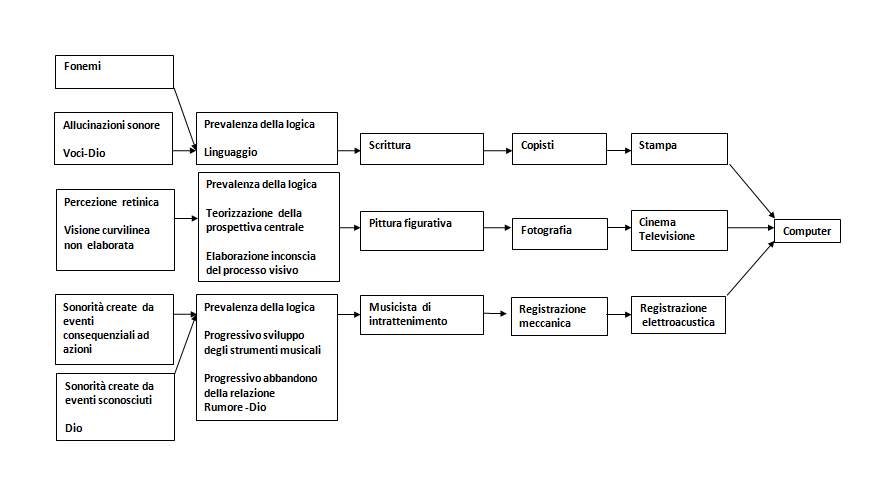
\includegraphics[width=0.99\columnwidth]{Graphics/foto/scheda_nuova}
\caption[]{}
\label{scheda}
\end{figure}
